% -*- latex -*-
%%%%%%%%%%%%%%%%%%%%%%%%%%%%%%%%%%%%%%%%%%%%%%%%%%%%%%%%%%%%%%%%
%%%%%%%%%%%%%%%%%%%%%%%%%%%%%%%%%%%%%%%%%%%%%%%%%%%%%%%%%%%%%%%%
%%%%
%%%% This text file is part of the source of 
%%%% `Introduction to High-Performance Scientific Computing'
%%%% by Victor Eijkhout, copyright 2012-2022
%%%%
%%%% This book is distributed under a Creative Commons Attribution 3.0
%%%% Unported (CC BY 3.0) license and made possible by funding from
%%%% The Saylor Foundation \url{http://www.saylor.org}.
%%%%
%%%%
%%%%%%%%%%%%%%%%%%%%%%%%%%%%%%%%%%%%%%%%%%%%%%%%%%%%%%%%%%%%%%%%
%%%%%%%%%%%%%%%%%%%%%%%%%%%%%%%%%%%%%%%%%%%%%%%%%%%%%%%%%%%%%%%%

Graph theory is the branch of mathematics that studies pairwise
relations between objects. Graphs both appear as tools for analyzing
issues in \ac{HPC}, and as objects of study themselves. This
appendix introduces the basic concepts and some relevant theory.

\Level 0 {Definitions}

A graph consists of a set of objects, and set of relations between them.
The objects, called the \emph{nodes}\index{node!in graph}
or \indexterm{vertices} of the graph, usually form a finite set, so we
usually identify them with consecutive integers $1\ldots n$ or $0\ldots
n-1$. The relation that holds between nodes is described by the
\indexterm{edges} of the graph: if $i$ and~$j$ are related, we say
that $( i,j)$ is an edge of the graph. This relation does not need to
be symmetric, take for instance the `less than' relation.

Formally, then, a graph is a tuple $G=\langle V,E\rangle$ where
$V=\{1,\ldots n\}$ for some~$n$, and $E\subset\{(i,j)\colon 1\leq
i,j\leq n,\,i\not=j\}$.

\begin{figure}[ht]
  \hbox{$\vcenter{\hbox{%pyskip
        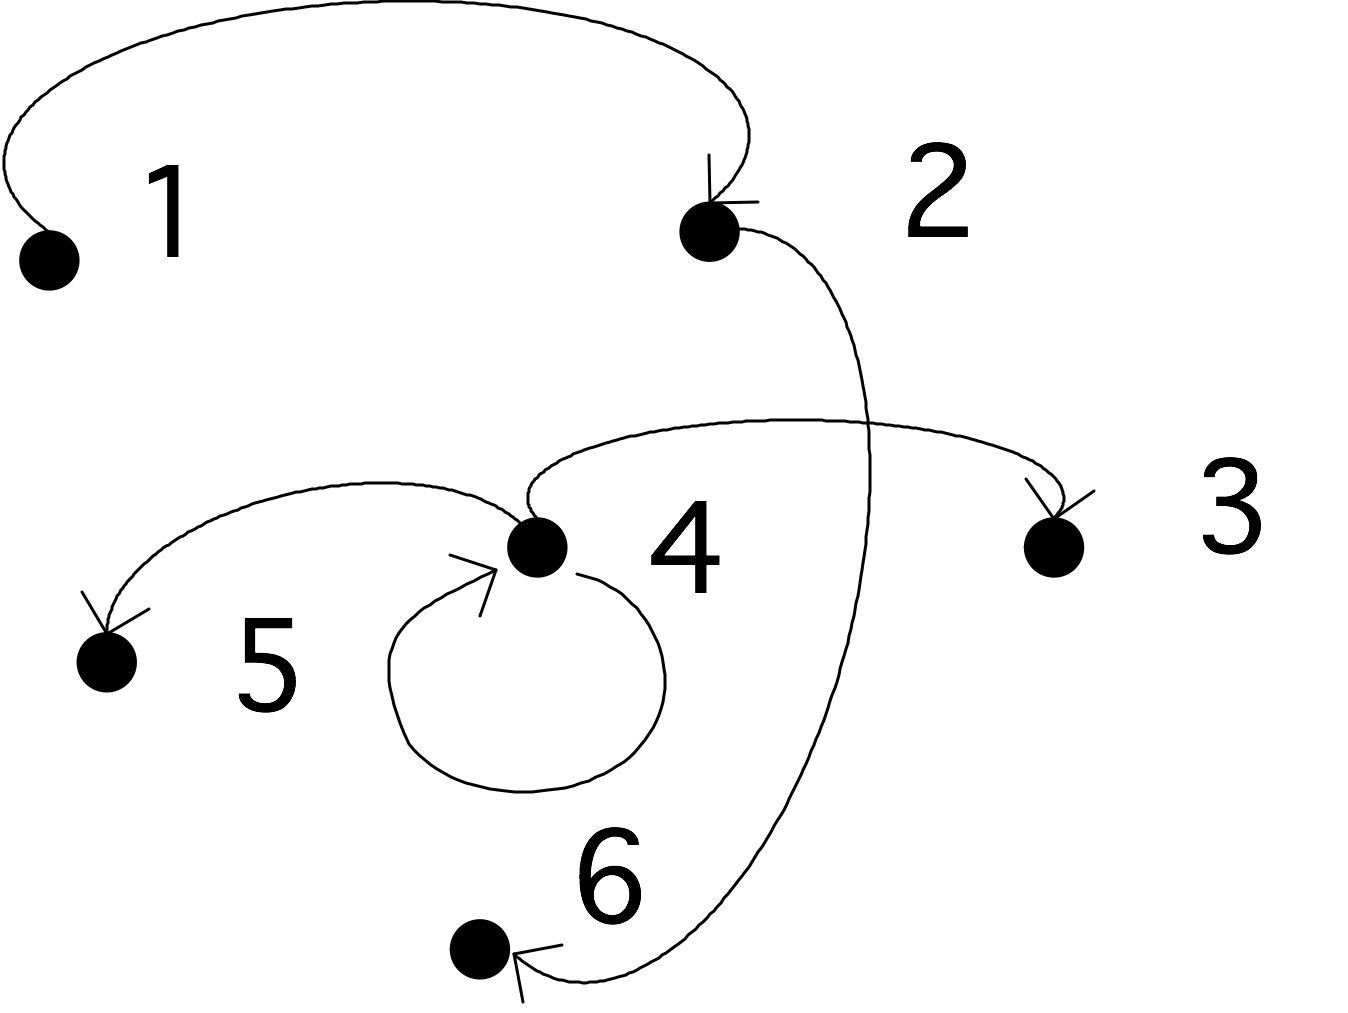
\includegraphics[scale=.1]{graph1}
    }}$%pyskip
    $
    \begin{cases}
      V=\{1,2,3,4,5,6\}\\
      E=\{ (1,2),(2,6),(4,3),(4,4),(4,5)\}
    \end{cases}
    $}
  \caption{A simple graph.}
  \label{fig:graph1}  
\end{figure}

A graph is called an \indextermsub{undirected}{graph} if $(i,j)\in
E\Leftrightarrow (j,i)\in E$. The alternative is a
\indextermsub{directed}{graph}, where we indicate an edge $(i,j)$ with
an arrow from $i$ to~$j$.

Two concepts that often appear in graph theory are the
degree and the diameter of a graph. 

\begin{definition}
The
\indexterm{degree} denotes the maximum number of nodes that are
connected to any node:
\[ 
  d(G)\equiv \max_i 
  \left|\{j\colon j\not=i\wedge (i,j)\in E\}\right|.
\]
\end{definition}

\begin{definition}
The \indexterm{diameter} of a graph is the length of the longest
shortest path
in the graph, where a \emph{path}\index{path (graph theory)}
is defined as a set of vertices
$v_1,\ldots, v_{k+1}$ such that $v_i\not=v_j$ for all $i\not=j$ and
\[ \forall_{1\leq i\leq k}\colon (v_i,v_{i+1})\in E. \]
The length of this path is~$k$.
\end{definition}
The concept of diameter is illustrated
in figure~\ref{fig:graph2}.

\begin{figure}[ht]
  \hbox{$\vcenter{\hbox{%pyskip
        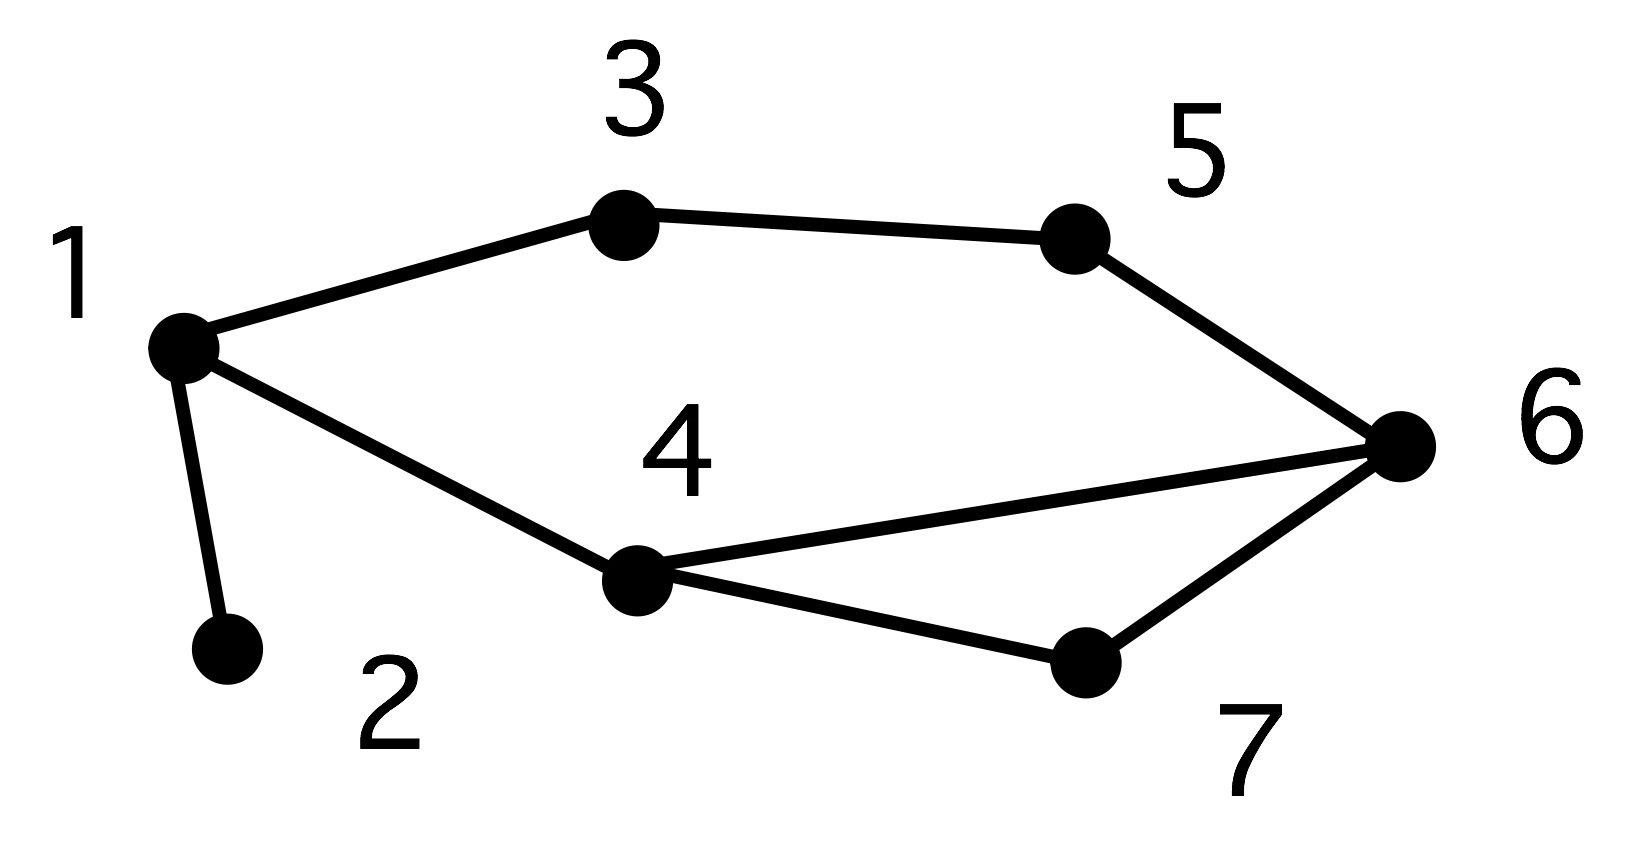
\includegraphics[scale=.1]{graph2a}
    }}$%pyskip
    A graph}
  \hbox{$\vcenter{\hbox{%pyskip
        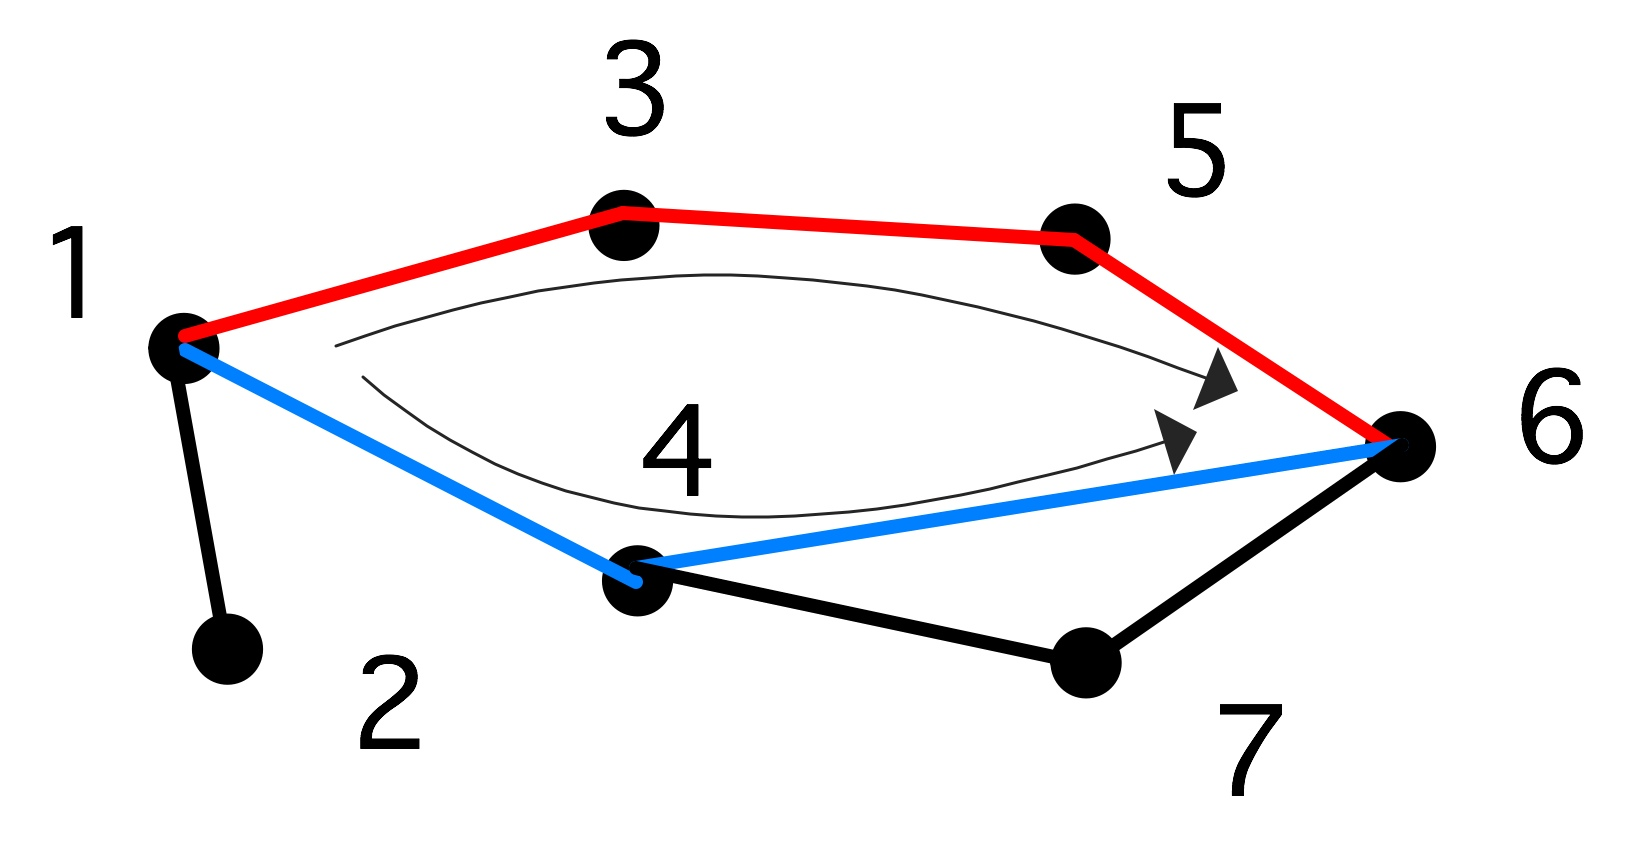
\includegraphics[scale=.1]{graph2b}
    }}$%pyskip
    Two paths from 1 to 6; $\langle 1,4,6\rangle$ is the shorter}
  \hbox{$\vcenter{\hbox{%pyskip
        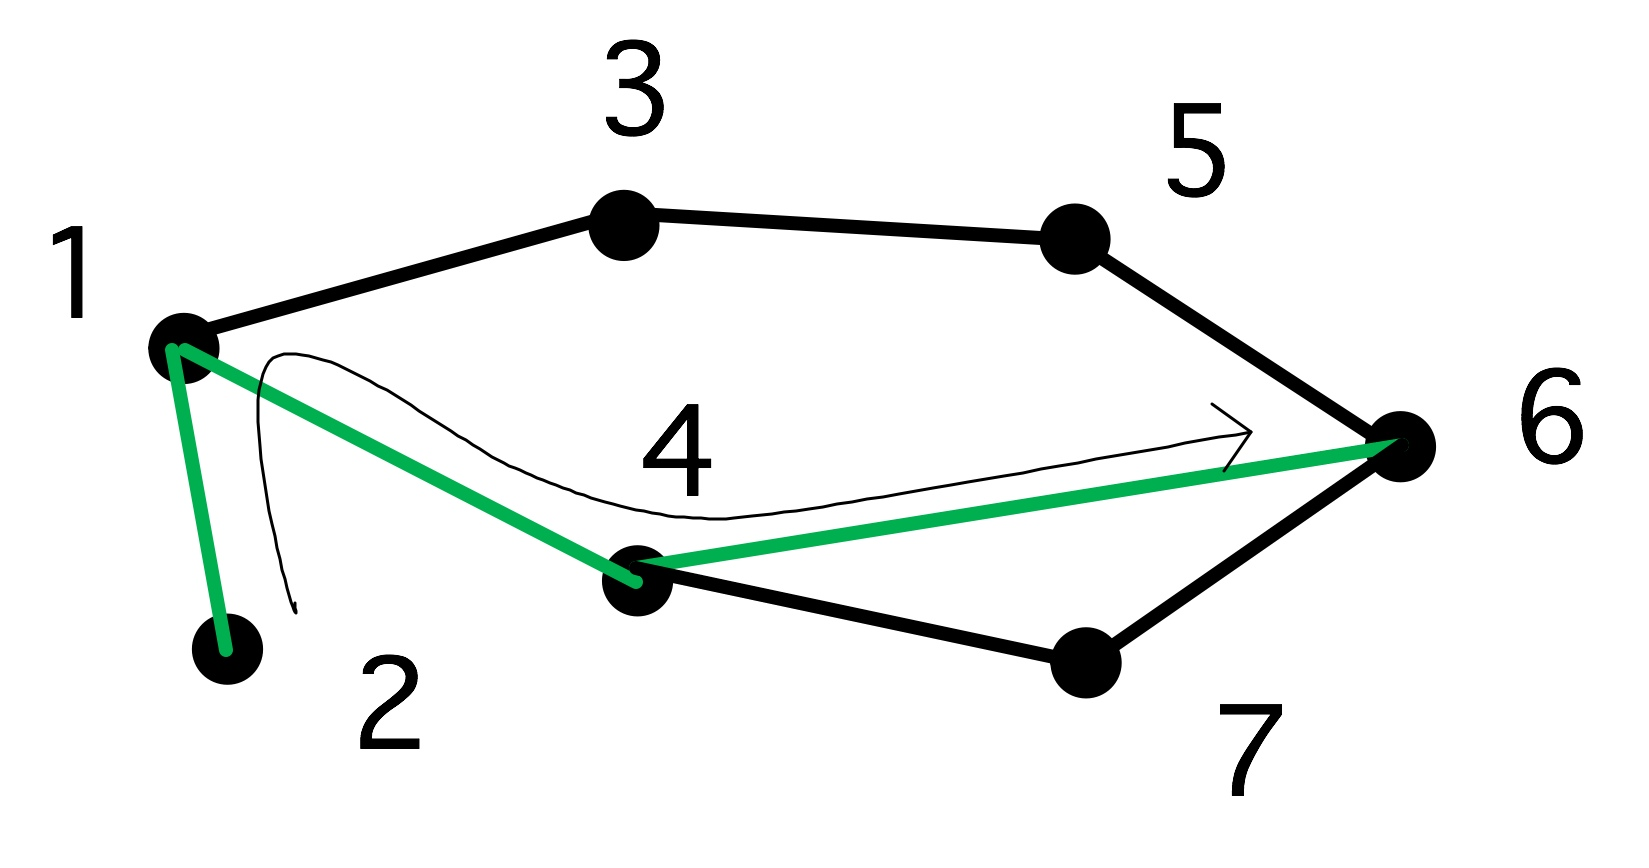
\includegraphics[scale=.1]{graph2c}
    }}$%pyskip
    The longest shortest path of this graph}
  \caption{Shortest paths.}
  \label{fig:graph2}
\end{figure}

A~path where all nodes are disjoint
except for $v_1=v_{k+1}$ is called a \emph{cycle}\index{cycle (in graph)}.

Sometimes we are only interested in the mere existence of an edge
$(i,j)$, at other times we attach a value or `weight' $w_{ij}$ to that
edge.
A~graph with weighted edges is called a \indextermsubdef{weighted}{graph}%
\index{weighted graph|see{graph, weighted}}.
Such a graph can be represented as a tuple
$G=\langle V,E,W\rangle$ where $E$ and $W$ have the same cardinality.
Conversely, an \indextermsubdef{unweighted}{graph}%
\index{unweighted graph|see{graph, unweighted}}
has all weights the same value, in which case we omit mention of weights.

\Level 0 {Common types of graphs}

\Level 1 {Directed Acyclic Graphs}

A graph that does not have cycles is called an
\indextermsubdef{acyclic}{graph}\index{acyclic graph|see{graph, acyclic}}
A special case of this type of graph is the \indexacf{DAG}.
This type of graph can for instance be
used to model dependencies between tasks:
if there is an edge from $i$ to~$j$,
it means that task $i$ has to be done before task~$j$.

\Level 1 {Trees}

One special case of \acp{DAG} is the
\indextermsubdef{tree}{graph}\index{tree graph|see{graph, tree}},
or for short a
\indextermdef{tree}\index{tree|seealso{graph, tree}}:
here any node can have multiple outgoing edges,
but only one incoming edge.
Nodes with no outgoing edges are \indexterm{leaf nodes};
a~node with no incoming edges is called a root,
and all other nodes are called \indexterm{interior nodes}.

\begin{exercise}
 Can a tree have more than one root?
\end{exercise}

\Level 1 {Separable graphs}

A
\indextermsubdef{separable}{graph}\index{separable graph|see{graph, separable}}
is a graph consisting of two sets of nodes,
where all connections are inside either of the sets.
Such graph can obviously be processed in parallel,
so several parallelization algorithms are concerned
with transforming a graph to a separable one.
If a graph can be written as $V=V_1+V_2+S$,
where nodes in~$V_1,V_2$ are only connected to~$S$,
but not to the other set,
we call $S$~a \indextermdef{separator}.

\Level 1 {Bipartite graphs}
\label{app:bipartite}

If a graph can be partitioned into two sets of nodes,
where edges only run from the one set to the other,
but not inside a set,
we call this a \indextermsubdef{bipartite}{graph}%
\index{bipartite graph|see{graph, bipartite}}.

\Level 0 {Graph colouring and independent sets}
\label{sec:independent}
\index{graph!colouring|(}

We can assign labels to the nodes of a graph, which is equivalent to
partitioning the set of nodes into disjoint subsets. One type of
labeling that is of interest is \emph{graph colouring}: here the
labels (or `colours') are chosen so that, if nodes $i$ and~$j$ have
the same colour, there is no edge connecting them: $(i,j)\not\in
E$. 

There is a trivial colouring of a graph, where each node has its own
colour. More interestingly,
the minimum number of colours with which you can colour a graph is
called the \indexterm{colour number} of the graph.

\begin{exercise}
  Show that, if a graph has degree~$d$, the colour number is at
  most~$d+1$.
\end{exercise}

A~famous graph colouring problem is the `four colour theorem': if
a graph depicts countries on a two-dimensional map (a so-called
`planar' graph), then the colour number is at most four.
In general, finding the colour number is hard (in fact, NP-hard).

The colour sets of a graph colouring are also called
\indexterm{independent sets}, since within each colour no node is
connected to a node of the same colour.

There is a trivial way of finding independent sets: declare each node
to have its own unique colour. On the other hand, finding the `best'
division in independent sets, for instance through finding the colour
number of the graph, is difficult. However, often it is enough to find
a reasonable partitioning of the nodes into independent sets, for
instance in constructing paralell ILU preconditioners;
section~\ref{sec:parallel-ilu}. The following algorithm does
that~\cite{jopl94,Luby:parallel}:
\begin{itemize}
\item Give each node a unique random number.
\item Now find the set of nodes that have a higher number than all of
  their neighbours; call this the first independent set.
\item Remove this set from the graph, and find again the nodes with a
  higher number than all their neighbours; this will be the second
  set.
\item Repeat this procedure until all nodes are in an independent set.
\end{itemize}
\begin{exercise}
  Convince yourself that the sets found this way are indeed independent.
\end{exercise}

\index{graph!colouring|)}

\Level 0 {Graph algorithms}

In this section we only briefly touch on graph algorithms; a full
discussion can be found in section~\ref{sec:graph-alg}.

\begin{itemize}
\item Distance algorithms. In applications such as traffic routing it
  is of interest to know the shortest distance from a given node to
  all others: the \indextermsub{single source}{shortest path} problem;
  or the shortest distance for any pair: the
  \indextermsub{all-pairs}{shortest path} problem.
\item Connectivity algorithms. In social networks it is of interest to
  know if two people are connected at all, if the graph can be split
  up into unconnected subgraphs, or whether some person is the crucial
  bridge between two groups.
\end{itemize}

\Level 0 {Graphs and matrices}
\label{sec:adj-matrix}
\index{matrix!adjacency|see{adjacency, matrix}}
\index{graph!adjacency|see{adjacency, graph}}

A graph can be rendered in a number of ways. You could of course just
list nodes and edges, but little insight can be derived that way.
Simple graphs can be  visualized by drawing vertices and edges, but
for large graphs this becomes unwieldy. Another option is to construct
the \indextermbusdef{adjacency}{matrix} of the graph.
For a graph $G=\langle V,E\rangle$,
the adjacency matrix $M$ (with a size $n$ equal to the
number of vertices~$|V|$) is defined by
\[ 
  M_{ij}=
  \begin{cases}1&(i,j)\in E\\ 0&\mbox{otherwise}\end{cases}
\]
Conversely, if you have a matrix, especially a
\indextermbus{sparse}{matrix}, you can construct its
\indextermbus{adjacency}{graph}.
This is illustrated in figure~\ref{fig:matrix-graph} for
\begin{figure}[ht]
  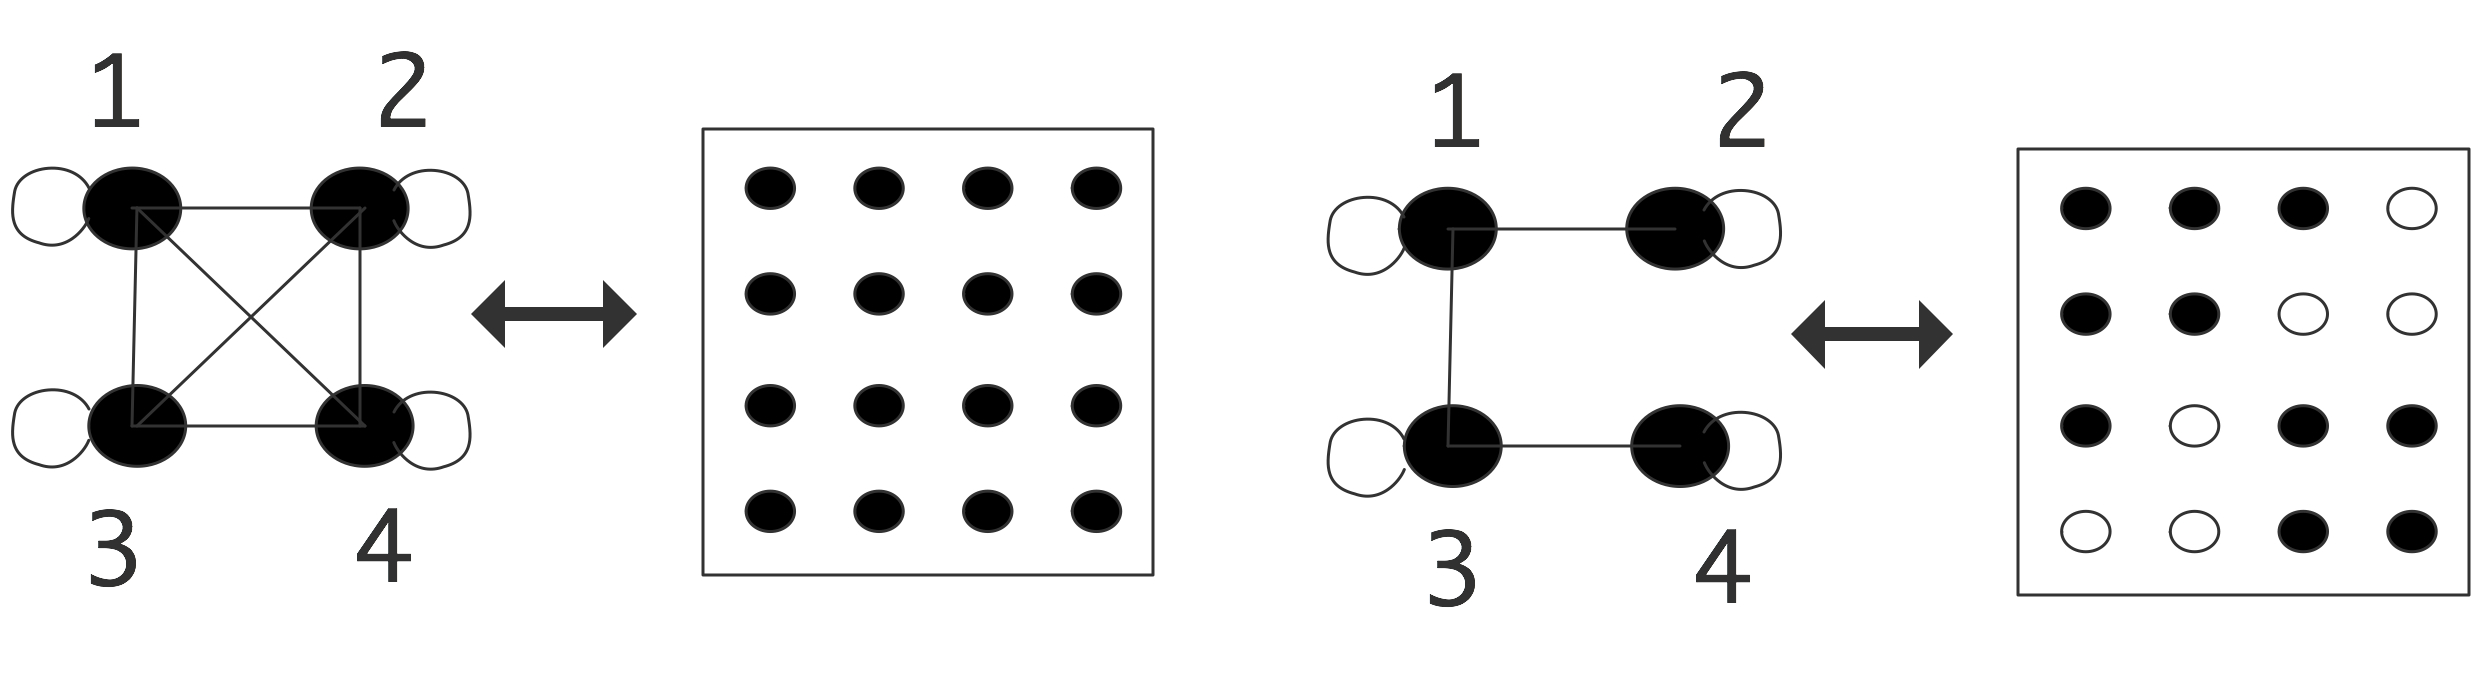
\includegraphics[scale=.14]{matrix-graph}
  \caption{A dense and a sparse matrix, both with their adjacency
    graph.}
  \label{fig:matrix-graph}
\end{figure}
both a dense and a sparse matrix. In this example, the matrices are
structurally symmetric, so we use lines instead of arrows in the
graphs. There is an edge on each vertex corresponding to the diagonal
element; this edge will often be left out of illustrations.

For graphs with edge weights, we set the elements of the adjacency
matrix to the weights:
\[ 
  M_{ij}=
  \begin{cases}w_{ij}&(i,j)\in E\\ 0&\mbox{otherwise}\end{cases}
\]

If a matrix has no zero elements, its adjacency graph has an edge
between each pair of vertices. Such a graph is called a
\indexterm{clique}.
If the graph is undirected, the adjacency matrix is symmetric, and
conversely, if a matrix is \indexterm{structurally symmetric}, its
adjacency graph is undirected.

\Level 1 {Permutation}

Graphs are often used to indicate relations between objects in the 
real world. One example would be `friend-of' relations in Facebook.
In such cases, the nodes in a graph do not have a natural numbering:
they are identified by a name, and any numbering is artificial.
Thus, we could wonder which graph properties remain invariant,
and which ones change, if we apply a different numbering.

Renumbering a set of objects can be modeled algebraically by
multiplying the adjacency matrix by a \indextermsub{permutation}{matrix}.
\begin{definition}
A permutation matrix is a square matrix where each row and column
has exactly one element equal to~one; all other elements are zero.
\end{definition}

\begin{exercise}
Let a set of $N$ objects $x_1,\ldots,x_N$ be given. What is the 
permutation matrix that orders them as $x_1,x_3,\ldots,x_2,x_4,\ldots$?
That is, find the matrix $P$ such that
\[
\begin{pmatrix}
x_1\\x_3\\\vdots\\x_2\\x_4\\\vdots
\end{pmatrix} = P
\begin{pmatrix}
x_1\\\vdots\\x_N
\end{pmatrix}
\]
\end{exercise}

\begin{exercise}
Show that the eigenvalues of a matrix are invariant under permutation.
\end{exercise}

\Level 1 {Irreducibility}

As an example of a graph concept that has an easy interpretation in the
adjacency matrix, consider reducibility.

\begin{definition}
A (directed) graph is called \indexterm{irreducible} if for every pair $i,j$ of
nodes there is a path from $i$ to~$j$ and from $j$ to~$i$. A~graph is
reducible if it is not irreducible.
\end{definition}

\begin{exercise}
  Let $A$ be a matrix
  \begin{equation}
    A=
    \begin{pmatrix}
      B&C\\ \emptyset&D
    \end{pmatrix}
    \label{eq:reduct-u}
  \end{equation}
  where $B$ and $D$ are square matrices. Prove the reducibility of the
  graph of which this is the adjacency matrix.
\end{exercise}

The matrix in equation~\ref{eq:reduct-u}
is block upper triangular matrix.
This means that solving a system $Ax=b$ is solved
in two steps, each of size~$N/2$, if $N$~is the size of~$A$.

\begin{exercise}
  Show that this makes the arithmetic complexity
  of solving $Ax=b$ lower than for a general $N\times N$ matrix.
\end{exercise}

If we permute a graph, its reducibility or irreducibility is not
changed. However, it may now no longer be apparent from looking 
at the adjacency matrix.

\Level 1 {Graph closure}
\label{app:graph-closure}

Here is another example of how adjacency matrices can simplify
reasoning about graphs.

\begin{definition}
  Let $G=\langle V,E\rangle$ be an undirected graph,
  then we define the closure of $G$ as $G'=\langle  V,E'\rangle$
  be the graph with the same vertices, but with vertices
  defined by
  \[ (i,j)\in E'\Leftrightarrow \exists_k\colon (i,k)\in E\wedge
  (k,j)\in E. \]
\end{definition}

As a small example:\\
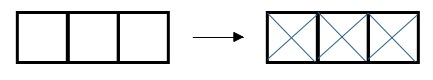
\includegraphics{graphclosure}
  
\begin{exercise}
  If $M$ is the adjacency matrix of~$G$, show that $M^2$ is the
  adjacency matrix of~$G'$, where we use boolean multiplication on the
  elements: $1\cdot1=1$, $1+1=1$.
\end{exercise}

\Level 0 {Spectral graph theory}
\label{app:fiedler}

With a graph $G$\footnote{This section owes much to Dan Spielman's course
on spectral graph theory~\url{http://www.cs.yale.edu/homes/spielman/561/}.}
and its adjacency matrix~$A_G$, we can define a
\indexterm{stochastic matrix} or \indextermbus{Markov}{matrix} by scaling
$A_G$ to have unit row sums:
\[ W_G = D_G\inv A_G\qquad \hbox{where $(D_G)_{ii}=\deg(i)$}. \]
To see how we interpret this, let's look at a simple example.
Let's take an unweighted graph with an adjacency matrix
\[
A_G = \begin{pmatrix}
1& &1&1\\
 & &1&1\\
1& &1&1\\
 &1&1& \\
\end{pmatrix}
\]
and look at the second row, which says that there are edges $(2,3)$ 
and $(2,4)$. This means that if you are on node~2, you can go 
to nodes 3 and~4. Scaling this matrix we get
\[
W_G = \begin{pmatrix}
1/3&   &1/3&1/3\\
   &   &1/2&1/2\\
1/3&   &1/3&1/3\\
   &1/2&1/2&   \\
\end{pmatrix}
\]
and now the second row says that from node~2 you can get
with equal probability to nodes 3 and~4.
You can also derive this statement mathematically:
\[
\begin{pmatrix}
0&1&0&0
\end{pmatrix} W_G =
\begin{pmatrix}
  0&  0&1/2&1/2\\
\end{pmatrix}
\]
It is simple to extrapolate that: if $p$ is a vector where the $i$-th
component gives the probability of being in node~$i$, then $(p^tW_G)_i$
is the probability of being in node~$i$ if you take one more
step along a graph edge.

\begin{exercise}
Prove that $p^tW_G$ is indeed a vector of probabilities. Hint: 
you can express that $p$ is a probability vector as $p^te=e$,
where $e$ is the vector of all ones.
\end{exercise}

\Level 1 {The graph Laplacian}
\label{sec:graph-laplace}

Another matrix to associate with a graph is the
\indextermbus{graph}{Laplacian}
\[ L_G = D_G-A_G. \]
This matrix has zero rowsums and positive diagonal entries, so by the
Gershgorin theorem (section~\ref{app:gershgorin} all its eigenvalues
are in the complex right half plane. 

\begin{exercise}
  Show that the vector of all ones is an eigenvector with eigenvalue~1.
\end{exercise}

This Laplacian matrix gives us a quadratic form:
\[ x^tL_Gx = \sum_{(i,j)\in E} (x_i-x_j)^2. \]

\Level 1 {Domain decomposition through Laplacian matrices}
\label{sec:fiedler-vector}

There are various interesting theorems connected with the graph
adjacency and Laplacian matrix. 
These have a very practical application to
\indexterm{domain decomposition}.

We get our inspiration of elliptic \acp{PDE}.

Connected with the \indexterm{Laplace equation}
$-\Delta u=f$ is an operator ${\cal L}u=-\Delta u$. 
On the unit interval $[0,1]$ the eigenfunctions
of this operator, that is, the functions for which ${\cal L}u=\lambda u$,
are $u_n(x)=\sin n\pi x$ for $n>0$. These have the property that $u_n(x)$
has $n-1$ zeros in the interior of the interval, and they divide the interval
in $n$ connected regions where the function is positive of negative.
Thus, if you wanted to divide a domain $\Omega$ over $p$ processors, you could
consider the $p$-th eigenfunction of the Laplacian on~$\Omega$, and find
the connected regions where it is positive or negative.

This statement about \ac{PDE} has a graph equivalent in two versions
of \indexterm{Fiedler's theorem}. (We will not give any proofs
in this section;
see~\cite{Spielman:spectral-graph-theory}.)
\begin{theorem}
  Let $G$ be a weighted path graph on $n$ vertices, let $L_P$ have
  eigenvalues $0 = \lambda_1 < \lambda_2\leq\ldots\leq\lambda_n$, and let
  $v_k$ be an eigenvector of~$\lambda_k$. Then $v_k$ changes sign
  $k-1$ times.
\end{theorem}

The second theorem is more useful~\cite{Fiedler:75-property}:
\begin{theorem}
  Let $G = (V,E,w)$ be a weighted connected graph, and let $L_G$ be
  its Laplacian matrix. Let $0 = \lambda_1 < \lambda_2 \leq \cdots
  \leq \lambda_n$ be the eigenvalues of $L_G$ and let $v_1,\ldots,v_n$
  be the corresponding eigenvectors. For any $k \geq 2$, let $W_k
  =\{i\in V\colon v_k(i)\geq0\}$. Then, the graph induced by $G$ on $W_k$
  has at most $k-1$ connected components.
\end{theorem}

The important consequence of this is that the eigenvector to the first
nontrivial eigenvalue can be used to partition the graph in two
connected piecesone of nodes where the eigenvector is positive, and
one where the eigenvector is negative. This eigenvector is known as
the \indextermdef{Fiedler vector}.
The adjacency matrix is nonnegative, and there is an extensive theory
for this type of matrix~\cite{BePl:book}; see the Perron-Frobenius
theorem in section~\ref{app:perron}.

In general there are no guarantees for how good a decomposition this
is, measured by the ratio of the numbers of edges, but in practice it
can be shown that the behaviour is pretty
good~\cite{Spielman96spectralpartitioning}.

%% \begin{lemma}
%%   The largest eigenvalue of the adjacency matrix can be bounded by the
%%   maximum node degree:
%%   \[ \alpha_1\leq d_{\max}. \]
%% \end{lemma}

\Level 1 {Cheeger's inequality}

Above we remarked that the first non-trivial eigenvalue of the graph
Laplacian has a relation to partitioning a graph in two parts. The
\indextermbus{Cheeger's}{constant} and
\indextermbus{Cheeger's}{inequality} relate this eigenvalue to a
certain quality measure of partitionings.

Let $V$ be the set of vertices and $S\subset V$, then Cheeger's
constant of a graph is defined as
\[ C=\min_S \frac{e(S,V-S)}
        {\min{\mathord{\mathrm{vol}}(S),\mathord{\mathrm{vol}}(V-S)}}
\]
where $e(S,V-S)$ denotes the number of edges connecting $S$ to $V-S$,
and the volume of a set of nodes is defined as
\[ \mathord{\mathrm{vol}}(S) = \sum_{e\in S}d(e). \]

Cheeger's inequality then states
\[ 2C \geq \lambda \geq \frac{C^2}2 \]
where $\lambda$ is the first nontrivial eigenvalue of the graph
Laplacian.

